\chapter{Application to Complex Problems}

We have seen how our architecture is adept at learning problems in the form of boolean functions. There are many problems, however, that cannot be easily modelled by such functions. This chapter will focus on applying the methods we have discussed to problems in image classification. Using the classical example of MNIST \cite{mnist}, an input image representing a handwritten digit from 0 to 9 is mapped to a probability distribution over all possible classifications. Deep learning proved to be very effective at this task \cite{mnist}. We hope to build an architecture that would be reasonably effective, while incorporating neurosymbolic elements that would allow us to interpret the learnt model.

\section{Architecture}

In Section \ref{section:lnns}, we discussed how the use of binary cross-entropy loss, as opposed to other loss functions, makes many boolean problems tractably learnable under the proposed architecture. The same reasoning applies to other forms of cross-entropy. If we have a well-trained MLP model for MNIST classification, and we aim to train a neurosymbolic model for the same problem, we can take the cross-entropy between the output distributions of the two models as an effective loss function.

We therefore construct an architecture as follows. Suppose we have dataset of pairs $[0,1]^D \times [0,1]^M$. Let $m, \psi$ represent models (with implicit parameters) $[0,1]^D \rightarrow [0,1]^M$, with $m$ being a traditional MLP model, and $\psi$ a neurosymbolic model. Define the \textit{difference loss} $\ell_d$ to be the cross entropy of the neurosymbolic model with respect to the MLP model, that is;
$$\ell_d(\vx) = \sum_{i=1}^M p_m(i) \cdot \log p_\psi(i)$$

Where $p_m$ is the vector $\text{softmax} \circ m(\vx)$ for input $\vx \in [0,1]^D$, and $p_\psi$ is the same for $\psi$. Our overall loss function would then take the form
$$\ell(\vx, y) = \sum_{i=1}^M \left[ \mathbbm{1}(y = i) \cdot \log p_m(i) \right] + \delta \ell_d(\vx)$$

for some hyperparameter $\delta > 0$. The first term is the traditional multi-class cross-entropy used to train any classification model, while the second term is the difference loss we have already discussed.

In MNIST, images are grids of size $28 \times 28$, making for $D=784$. Too many parameters would make our model more difficult to interpret, but by chaining the joint model multiple times, we can overcome this. Suppose we had pairs of models $(m_1, \psi_1), \dots, (m_n, \psi_n)$ defined similarly to before. A more general loss would then be defined by
$$
\begin{aligned}
\vz_0 &= \vx \\
\vz_i &= m_i(\vz_{i-1}) \text{ for all } i = 1, \dots, n \\
\ell(\vx, y) &= \sum_i \left[ \mathbbm{1}(y = i) \cdot \log \text{softmax}(\vz_n)(i) \right] + \delta \sum_{i=1}^n \ell_{d,i}(\vz_{i-1})
\end{aligned}
$$

where $\ell_{d,i}$ is the difference loss for the $i$th model pair $(m_i, \psi_i)$. The model we actually use has $n=2$ pairs of models. $m_1$ has no hidden layers, and has output dimension $128$. $m_2$ has one hidden layer of size $64$, before outputting values of size $M=10$. Every MLP model ends in a softmax function so that outputs are in the interval $[0,1]$, but for the remaining non-linearities, we use the ``LeakyReLU'' activation function \cite{leakyrelu}. We also replace the difference loss $\ell_{d,1}$ for the first pair with $\ell_2$ hinge loss on the MLP model $m_1$'s parameters;

$$
\begin{aligned}
\ell(\vx, y) &= \sum_i \left[ \mathbbm{1}(y = i) \cdot \log \text{softmax}(\vz_n)(i) \right] + \delta \ell_{d,2}(\vz_1) + \lambda \ell_2(m_1)
\end{aligned}
$$

where $\lambda > 0$ is another hyperparameter. This is done as $m_1$ is simply a generalised linear model, which is less difficult to interpret, as long as the model does not overfit to random noise, which we control using $\ell_2$ regularisation.

The neurosymbolic model $\psi_2$ is a series of $M=10$ DNF models under Schweizer-Sklar $p=-2$ logic, as described in Section \ref{section:realdnfs}. Each DNF model is the disjunction of 4 conjunctions over 128 input variables. We again fix the sign parameter $\vs$ to 0, as this aids in intepreting the result of the model, and we will show it does not significantly affect the rate of convergence.

\subsection{Results}

A good metric for the success of this model is the quality of the output of the neurosymbolic submodel. If we take the output distribution $\text{softmax} \circ \psi_2 \circ m_1 (\vx)$, and take the index of maximum probability as our true guess, comparing this to the actual categorisation over all images in the test dataset allows us to assess the quality of $\psi_2$. Interpretability requires that the parameters of $\psi_2$ be as crisp as possible, so we also consider the sum of the distances of all logical parameters from crisp values $0, 1$.

\begin{figure}[H]
    \centering
    \begin{subfigure}[t]{0.45\textwidth}
        \centering
        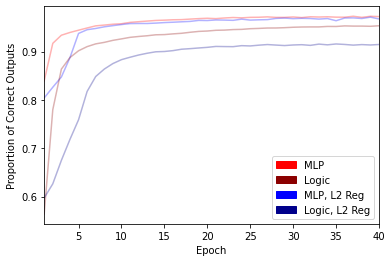
\includegraphics[width=\textwidth]{imgs/mnist-co.png}
        \caption{Proportion of Correct Outputs (for both MLP and neurosymbolic paths).}
        \label{fig:mnistco}
    \end{subfigure}
    \begin{subfigure}[t]{0.45\textwidth}
        \centering
        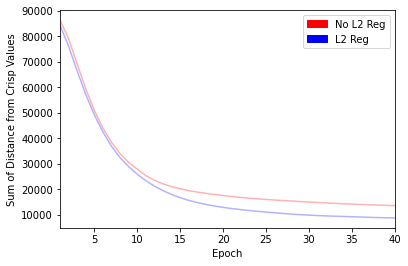
\includegraphics[width=\textwidth]{imgs/mnist-crispness.png}
        \caption{Sum of distances from crisp parameters $0,1$.}
        \label{fig:mnistcrispness}
    \end{subfigure}
    \begin{subfigure}[t]{0.45\textwidth}
        \centering
        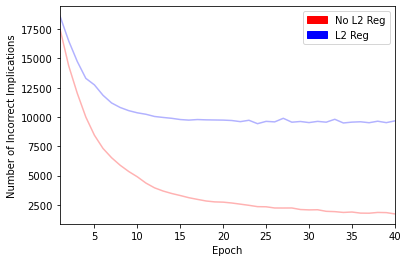
\includegraphics[width=\textwidth]{imgs/mnist-unsatisfied.png}
        \caption{Number of incorrect implications.}
        \label{fig:mnistunsatisfied}
    \end{subfigure}
    \begin{subfigure}[t]{0.45\textwidth}
        \centering
        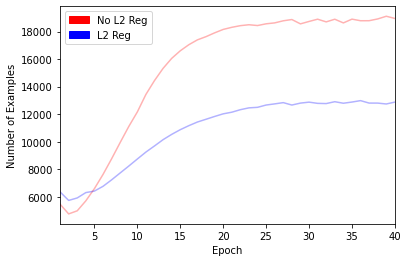
\includegraphics[width=\textwidth]{imgs/mnist-examples.png}
        \caption{Number of ``example'' implications.}
        \label{fig:mnistexamples}
    \end{subfigure}
       \caption{Convergence of the MNIST categorisation model, $\delta=10^{-1}$.}
       \label{fig:mnist}
\end{figure}

Figure \ref{fig:mnist} shows the results of optimising this model using Adam optimisation with a learning rate of $10^{-3}$. We set $\delta=10^{-1}$, and where $\ell_2$ loss is used, $\lambda = 10^{-5}$. Figure \ref{fig:mnistco} shows that the quality of predictions of the traditional MLP path does not degrade, achieving around 97\% accuracy in both cases. Non-zero $\ell_2$ regularisation diminishes the quality of the neurosymbolic prediction, but not significantly. Figure \ref{fig:mnistcrispness} shows that both models achieve relatively crisp parameters, with the average distance from $0,1$ decreasing by a factor of 10.  

Figure \ref{fig:mnistunsatisfied} and \ref{fig:mnistexamples} measure the effectiveness of $\psi_2$ in capturing logical inference though the implication operator $\limply$. A single DNF in $\psi_2$ is a disjunction of conjunctions $c_1 \lor \dots \lor c_n$, and we want this disjunction to be true if and only if the training data has the corresponding output $y$ true. If this is the case, then for all conjunctions $c_i$, $c_i \limply y$. If, for some element of the test dataset $\vx$, we have that $c_i$ is true, but $y$ is false, then our learnt conjunction is incorrect. If instead $y$ is true, we can interpret $c_i$ as \textit{causing} $y$ to be true. Figure \ref{fig:mnistunsatisfied} therefore represents the sum of $c_i \land \lnot y$ over all conjunctions $c_i$ and all test data pairs. Figure \ref{fig:mnistexamples} represents the sum of $c_i \land y$ likewise. We see that the number of incorrect implications decreases over time, and the number of ``example'' implications increases, before both plateauing after around 20 epochs. $\ell_2$ regularisation also diminishes the quality of both metrics, which is not surprising given the findings of \ref{fig:mnistco}. In Appendix \ref{section:moremnisttrain}, we further explore how varying the difference hyperparameter $\delta$ affects the quality of the resultant model.

\section{Model Interpretation}


\begin{wrapfigure}[27]{r}{0.45\linewidth}
    \centering
    \vspace{-35.0pt}
    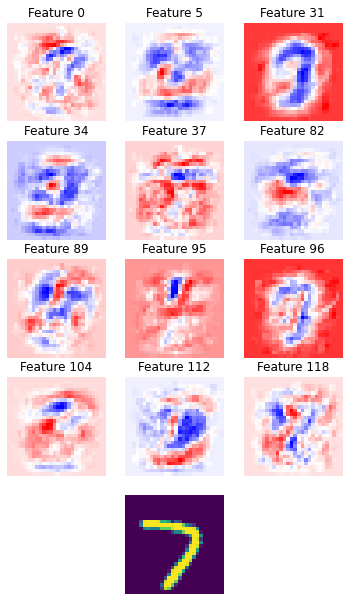
\includegraphics[width=0.35\textwidth]{imgs/interpret7.png}
    \vspace{10.0pt}
    \caption[width=0.3\textwidth]{The image is given label 7 as all the above features are true.}
    \label{fig:interpret7}
\end{wrapfigure}

The model we have designed has become quite adept at categorising MNIST images. The goal of this report, however, is to determine a method of interpreting said models. As before, we want to leverage the fact that a boolean statement in DNF can be considered a series of implications from conjunctions $c$ to outputs $y$. It is interesting to note that statements $c \limply y$ are known as \textit{Horn clauses}, and are a relatively small but highly expressive subset of boolean functions, which are widely used in symbolic learning algorithms, especially in ILP systems \cite{hornclause}. 

If for some DNF in $\psi_2$, the output $y$ is true, and one of the antecedent conjunctions $c$ is also true, then we interpret $c$ as causing $y$. We therefore need only explain why $c$ was true. In the model we have designed, $c$ is the output of a generalised linear model, so we can use Variable Importance Measures (VIMs), as discussed in Section \ref{section:vims}. 

Figure \ref{fig:interpret7} shows such an example. The listed features are elements of a conjunction $c$ which implies the output that gives the image label 7. Each image is generated by taking the gradient of the output feature in $\vz_1$ with respect to training image $\vx$. The example shown is from the model with $\ell_2$ hinge loss with hyperparameter $\lambda = 10^{-5}$. We can see that many of the features very closely map the shape of a number 7, and the remaining features capture small variances in said shape. This example was chosen as it required the conjunction with the fewest number of terms, more examples are given in Appendix \ref{section:moremnistinterp}. Of note is that feature attributions are much more difficult to comprehend without $\ell_2$ regularisation, as the model overfits to random noise around the borders of each image.

